% \iffalse
\let\negmedspace\undefined
\let\negthickspace\undefined
\documentclass[journal,12pt,twocolumn]{IEEEtran}
\usepackage{cite}
\usepackage{amsmath,amssymb,amsfonts,amsthm}
\usepackage{algorithmic}
\usepackage{graphicx}
\usepackage{textcomp}
\usepackage{xcolor}
\usepackage{txfonts}
\usepackage{listings}
\usepackage{enumitem}
\usepackage{mathtools}
\usepackage{gensymb}
\usepackage{comment}
\usepackage[breaklinks=true]{hyperref}
\usepackage{tkz-euclide}
\usepackage{listings}
\usepackage{gvv}
\def\inputGnumericTable{}
\usepackage[latin1]{inputenc}
\usepackage{color}
\usepackage{array}
\usepackage{longtable}
\usepackage{calc}
\usepackage{multirow}
\usepackage{hhline}
\usepackage{ifthen}
\usepackage{lscape}

\newtheorem{theorem}{Theorem}[section]
\newtheorem{problem}{Problem}
\newtheorem{proposition}{Proposition}[section]
\newtheorem{lemma}{Lemma}[section]
\newtheorem{corollary}[theorem]{Corollary}
\newtheorem{example}{Example}[section]
\newtheorem{definition}[problem]{Definition}
\newcommand{\BEQA}{\begin{eqnarray}}
\newcommand{\EEQA}{\end{eqnarray}}
\newcommand{\define}{\stackrel{\triangle}{=}}
\theoremstyle{remark}
\newtheorem{rem}{Remark}
\begin{document}

\bibliographystyle{IEEEtran}
\vspace{3cm}

\title{NCERT Discrete 10.5.2 -15}
\author{EE23BTECH11057 - Shakunaveti Sai Sri Ram Varun$^{}$% &lt;-this % stops a space
}
\maketitle
\newpage
\bigskip

\renewcommand{\thefigure}{\theenumi}
\renewcommand{\thetable}{\theenumi}
\vspace{2cm}
\textbf{Question: }
For what value of $ n$, are the $ nth$ terms of two A.Ps: 63, 65, 67,... and 3, 10, 17,... equal?\\
\vspace{0.5cm}
\textbf{Solution}:
A sequence is said to be in Arithmetic Progression when it is in the form of
\begin{align}
\notag a, a+d, a+2d, a+3d,....
\end{align}
where $a$ is first term and $d$ is common difference.\\
When there are $ n$ terms, the sequence becomes
\begin{align}
\notag a, a+d, a+2d, a+3d,....., a+(n-1)d.\\
\notag T_n = a+(n-1)d.
\end{align}
which is nth term.
In the given question, there are two sequences.
\begin{align}
63, 65, 67....\label{eq:1}\\
3, 10, 17....\label{eq:2}
\end{align}
let f(n) be unit step function.\\
\begin{align}
\text{i.e. f(n)}=
\begin{array}{lr}
    1,&\text{n}>=0\\
    0,&\text{n}<0
\end{array}
\end{align}
\begin{enumerate}
\item [(i)]
for the sequence $ \eqref{eq:1}$, let x(n) be $ nth$ term,
\begin{align}
\notag a = 63\\
\notag a+d = 65\\
\notag d = 2\\
\notag \text{x(n)} = 63 + (n-1)\times2\\
\text{x(n)} = 61 + 2n \label{eq:3}
\end{align}
\boxed{\text{x(n)} = 61\text{f(n-1)} + 2n\text{f(n-1)}}\\
\begin{figure}
    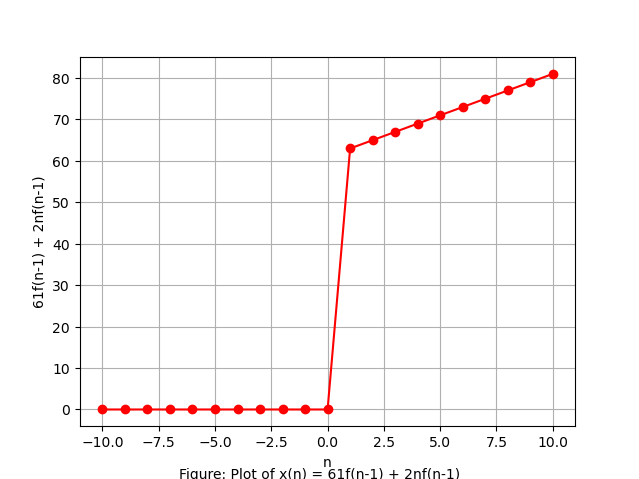
\includegraphics[width = 11cm]{Figure_1.png}
\end{figure}
\begin{align}
\text{To find X(z)(i.e. the 'z' transform)}:\\
\text{X(z)} = \sum_{n=-\infty}^{\infty} x(n)\times \text{z}^{-n}\\
\notag \text{X(z)} = \sum_{n=-\infty}^{\infty} (61\text{f(n-1)} + 2\text{nf(n-1)})\text{z}^{-n}\\
\text{X(z)} = \sum_{n=1}^{\infty} (61 + 2n)\text{z}^{-n} + 0
\end{align}
\begin{align}
\notag \text{X(z)} = \lim_{n\to\infty} [61(1-z^{-n})(z-1)^{-1}+ 2(z-1)^{-1}\\
+ 2(z^{n-1}-1)(z^{1-n})(z-1)^{-1}-2[(n-1)z+1]z^{n-1}]\\
\boxed{\text{X(z)} = 61(\text{z}-1)^{-1} + 2(2z-1)(z-1)^{-2}  \forall  |z|>1}
\end{align}
\item[(ii)]
for sequence $ \eqref{eq:2}$ , let y(n) be $ nth$ term,
\begin{align}
\notag a = 3 \\
\notag a+d = 10\\
\notag d = 7\\
\notag \text{y(n)} = 3 + (n-1)\times7\\
\text{y(n)} = 7n - 4 \label{eq:4}\\
\boxed{\text{y(n)} = -4\text{f(n-1)} + 7n\text{f(n-1)}}
\end{align}
\begin{figure}
    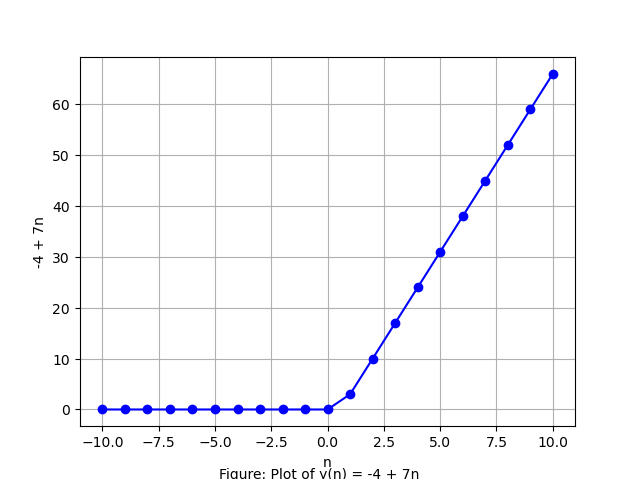
\includegraphics[width = 11cm]{Figure_2.png}
\end{figure}
To find Y(z) (the 'z' transform):\\
\begin{align}
\text{Y(z)} = \sum_{n=-\infty}^{\infty} y(n)\text{z}^{-n}\\
\notag \text{Y(z)} = \sum_{n=-\infty}^{\infty} (-4\text{f(n-1)} + 7n\text{f(n-1)})\text{z}^{-n}\\
\notag \text{Y(z)} = \sum_{n=1}^{\infty} (-4 + 7n)\text{z}^{-n} + 0\\
\notag \text{Y(z)} = \lim_{n\to\infty} [-4(1-z^{-n})(z-1)^{-1}+ 7(z-1)^{-1}\\
+ 7(z^{n-1}-1)(z^{1-n})(z-1)^{-1}-7[(n-1)z+1]z^{n-1}]\\
\boxed{\text{Y(z)} = -4(z-1)^{-1} + 7(2z-1)(z-1)^{-2} \forall  |z|>1}
\end{align}
given, x(n) = y(n)\\
\begin{align}
\therefore 61 + 2n = 7n -4\\
\notag 5n = 65\\
n = 13\\
\notag So, \text{x(n)} = 61 + 2\times13 = 87 \text{ and}\\
\notag \text{y(n)} = 7\times13 - 4 = 87
\end{align}
$ \therefore$ 13th terms of given two APs are equal.\\\\
\end{enumerate}
\end{document}
